\documentclass[conference]{IEEEtran}
\usepackage[T1]{fontenc}
\usepackage{newtxtext,newtxmath}  % Times-matched math, so numbers in formulas match the text
\usepackage{booktabs,graphicx,amsmath,array,multirow,xcolor,url}
\usepackage[hidelinks]{hyperref}
\usepackage{cite}
\graphicspath{{../results/figures/}}
% generated by src/11_report_assets.py -- do not edit by hand
\newcommand{\AgeOtherCoderabbit}{233}
\newcommand{\AgeOtherDevin}{348}
\newcommand{\AgeOwnCoderabbit}{403}
\newcommand{\AgeOwnDevin}{503}
\newcommand{\AmazonQDrop}{9.3}
\newcommand{\BTAriMax}{0.93}
\newcommand{\BTAriMin}{0.78}
\newcommand{\BTEff}{medium}
\newcommand{\BTReproMin}{5}
\newcommand{\BTResCodeRabbitCode}{12.2}
\newcommand{\BTV}{0.21}
\newcommand{\BTVMax}{0.21}
\newcommand{\BTVMin}{0.21}
\newcommand{\ChiAttribution}{4{,}315.7}
\newcommand{\ChiLabelled}{526.1}
\newcommand{\ChiLanguage}{424.7}
\newcommand{\ChiReason}{73.4}
\newcommand{\ChiState}{214.8}
\newcommand{\ClosedMax}{79.9}
\newcommand{\ClosedMaxAgent}{Gemini Code Assist}
\newcommand{\ClosedMaxCI}{[74.6, 84.4]}
\newcommand{\ClosedMin}{36.4}
\newcommand{\ClosedMinAgent}{Amazon Q}
\newcommand{\ClosedMinCI}{[27.9, 45.9]}
\newcommand{\ClosedRankAider}{7}
\newcommand{\ClosedRankAmazonQ}{6}
\newcommand{\ClosedRankClaudeCode}{2}
\newcommand{\ClosedRankCoderabbit}{11}
\newcommand{\ClosedRankDevin}{8}
\newcommand{\ClosedRankGeminiCodeAssist}{5}
\newcommand{\ClosedRankJules}{10}
\newcommand{\ClosedRankKiro}{9}
\newcommand{\ClosedRankPrAgent}{1}
\newcommand{\ClosedRankSweAgent}{4}
\newcommand{\ClosedRankSweep}{3}
\newcommand{\CodeRabbitOwnPRRef}{92.2}
\newcommand{\CodeShareOtherCodeRabbit}{20.1}
\newcommand{\CodeShareOwnCodeRabbit}{45.3}
\newcommand{\CodeTopicShareCodeRabbit}{67.6}
\newcommand{\CvMax}{0.51}
\newcommand{\CvMin}{0.47}
\newcommand{\DeltaMax}{\ensuremath{-}0.44}
\newcommand{\DiffCICoderabbit}{[\ensuremath{-}23.5, \ensuremath{-}12.6]}
\newcommand{\DiffCIDevin}{[\ensuremath{-}32.5, \ensuremath{-}13.6]}
\newcommand{\DiffCoderabbit}{\ensuremath{-}18.3}
\newcommand{\DiffDevin}{\ensuremath{-}23.9}
\newcommand{\DiffOldCoderabbit}{\ensuremath{-}18.1}
\newcommand{\DiffOldDevin}{\ensuremath{-}24.8}
\newcommand{\DocShareCodeRabbit}{43.7}
\newcommand{\DomFFive}{871}
\newcommand{\DomFFour}{1{,}140}
\newcommand{\DomFOne}{804}
\newcommand{\DomFThree}{479}
\newcommand{\DomFTwo}{522}
\newcommand{\DomHOne}{3{,}231}
\newcommand{\DomHTwo}{585}
\newcommand{\EchoAmazonq}{33.6}
\newcommand{\EffAttribution}{large}
\newcommand{\EffLabelled}{medium}
\newcommand{\EffLanguage}{small}
\newcommand{\EffReason}{small}
\newcommand{\EffState}{small}
\newcommand{\EffTFFive}{small}
\newcommand{\EffTFMain}{large}
\newcommand{\EffTFSThree}{medium}
\newcommand{\EffTFSTwo}{medium}
\newcommand{\EffTFStable}{medium}
\newcommand{\EffTHFive}{small}
\newcommand{\EffTHMain}{small}
\newcommand{\EffTHSThree}{small}
\newcommand{\EffTHSTwo}{small}
\newcommand{\EpsCompleted}{0.097}
\newcommand{\EpsFine}{0.20}
\newcommand{\EpsHeadline}{0.15}
\newcommand{\EpsNotPlanned}{0.062}
\newcommand{\EpsSFour}{0.082}
\newcommand{\EpsSOne}{0.083}
\newcommand{\EpsSThree}{0.092}
\newcommand{\EpsSTwo}{0.045}
\newcommand{\GiniMax}{0.40}
\newcommand{\GiniMaxAgent}{Devin}
\newcommand{\GiniMin}{0.04}
\newcommand{\GiniMinAgent}{Aider}
\newcommand{\HCoderabbit}{0.39}
\newcommand{\HDevin}{0.51}
\newcommand{\HEffCoderabbit}{small}
\newcommand{\HEffDevin}{medium}
\newcommand{\JulesDrop}{10.2}
\newcommand{\KMAider}{79.7}
\newcommand{\KMAmazonQ}{not reached}
\newcommand{\KMClaudeCode}{1.1}
\newcommand{\KMCoderabbit}{138.9}
\newcommand{\KMDaysCode}{83.1}
\newcommand{\KMDaysWorkflow}{10.3}
\newcommand{\KMDevin}{181.2}
\newcommand{\KMGeminiCodeAssist}{4.8}
\newcommand{\KMJules}{7.0}
\newcommand{\KMKiro}{17.8}
\newcommand{\KMPrAgent}{152.9}
\newcommand{\KMRankAider}{7}
\newcommand{\KMRankAmazonQ}{11}
\newcommand{\KMRankClaudeCode}{1}
\newcommand{\KMRankCoderabbit}{8}
\newcommand{\KMRankDevin}{10}
\newcommand{\KMRankGeminiCodeAssist}{3}
\newcommand{\KMRankJules}{4}
\newcommand{\KMRankKiro}{5}
\newcommand{\KMRankPrAgent}{9}
\newcommand{\KMRankSweAgent}{2}
\newcommand{\KMRankSweep}{6}
\newcommand{\KMSweAgent}{4.8}
\newcommand{\KMSweep}{29.5}
\newcommand{\KWH}{266.4}
\newcommand{\KWdf}{10}
\newcommand{\KWeff}{medium}
\newcommand{\KWeps}{0.082}
\newcommand{\KWp}{2.0\times10^{-51}}
\newcommand{\LRchi}{394.0}
\newcommand{\LRp}{1.8\times10^{-78}}
\newcommand{\LabelsMeanMax}{2.01}
\newcommand{\LabelsMeanMaxAgent}{Amazon Q}
\newcommand{\LabelsMeanMin}{0.55}
\newcommand{\LabelsMeanMinAgent}{PR-Agent}
\newcommand{\MaxPctSparse}{36}
\newcommand{\MedAider}{67.4}
\newcommand{\MedAmazonQ}{61.0}
\newcommand{\MedCIAider}{[13.9, 279.2]}
\newcommand{\MedCIAmazonQ}{[22.9, 306.3]}
\newcommand{\MedCIClaudeCode}{[7.4, 15.7]}
\newcommand{\MedCICoderabbit}{[152.2, 252.2]}
\newcommand{\MedCIDevin}{[48.0, 160.7]}
\newcommand{\MedCIGeminiCodeAssist}{[17.8, 71.4]}
\newcommand{\MedCIJules}{[45.8, 179.5]}
\newcommand{\MedCIKiro}{[29.0, 339.4]}
\newcommand{\MedCIPrAgent}{[1.1, 50.1]}
\newcommand{\MedCISweAgent}{[16.8, 57.9]}
\newcommand{\MedCISweep}{[11.9, 36.8]}
\newcommand{\MedClaudeCode}{11.1}
\newcommand{\MedCoderabbit}{180.3}
\newcommand{\MedDevin}{75.0}
\newcommand{\MedGeminiCodeAssist}{34.5}
\newcommand{\MedJules}{109.3}
\newcommand{\MedKiro}{105.0}
\newcommand{\MedPrAgent}{9.5}
\newcommand{\MedSweAgent}{26.6}
\newcommand{\MedSweep}{22.5}
\newcommand{\MedTokens}{65}
\newcommand{\MedianTTCAll}{51.1}
\newcommand{\MedianTTCTested}{50.6}
\newcommand{\NActionsEcho}{134}
\newcommand{\NAgents}{13}
\newcommand{\NAgentsNotPlanned}{6}
\newcommand{\NBot}{2{,}278}
\newcommand{\NClosed}{3{,}275}
\newcommand{\NDigest}{6}
\newcommand{\NDigestInSThree}{1}
\newcommand{\NDocsRQThree}{3{,}816}
\newcommand{\NDup}{30}
\newcommand{\NEnglish}{4{,}209}
\newcommand{\NEnglishTested}{4{,}203}
\newcommand{\NInstant}{47}
\newcommand{\NIssues}{4{,}952}
\newcommand{\NLabelsDistinct}{1{,}345}
\newcommand{\NLatinNonEn}{48}
\newcommand{\NNonLatin}{695}
\newcommand{\NNonNormalLog}{9}
\newcommand{\NOpen}{1{,}677}
\newcommand{\NOtherCoderabbit}{299}
\newcommand{\NOtherDevin}{99}
\newcommand{\NOverYear}{119}
\newcommand{\NOwnBot}{2{,}091}
\newcommand{\NOwnCoderabbit}{1{,}643}
\newcommand{\NOwnDevin}{439}
\newcommand{\NPR}{18}
\newcommand{\NPairsLarge}{0}
\newcommand{\NPairsMedium}{5}
\newcommand{\NPairsNegligible}{28}
\newcommand{\NPairsSmall}{22}
\newcommand{\NPreRelease}{10}
\newcommand{\NRQTwo}{3{,}269}
\newcommand{\NRaw}{5{,}000}
\newcommand{\NRepos}{3{,}466}
\newcommand{\NReposRaw}{3{,}477}
\newcommand{\NReposSFour}{2{,}358}
\newcommand{\NSThree}{4{,}591}
\newcommand{\NSelfRef}{189}
\newcommand{\NSig}{13}
\newcommand{\NTemplateLines}{17{,}654}
\newcommand{\NTopicsF}{5}
\newcommand{\NTopicsH}{2}
\newcommand{\NVocab}{3{,}088}
\newcommand{\NonEnAider}{4.4}
\newcommand{\NonEnClaudeCode}{20.3}
\newcommand{\NonEnCoderabbit}{12.0}
\newcommand{\NonEnDevin}{33.8}
\newcommand{\NonEnGeminiCodeAssist}{33.1}
\newcommand{\NonEnSweep}{2.2}
\newcommand{\OtherCICoderabbit}{[70.1, 79.8]}
\newcommand{\OtherCIDevin}{[67.5, 84.0]}
\newcommand{\OtherClosedAll}{73.5}
\newcommand{\OtherClosedCoderabbit}{75.3}
\newcommand{\OtherClosedDevin}{76.8}
\newcommand{\OtherMaxDrop}{1.5}
\newcommand{\OwnBotShareCoderabbit}{84.6}
\newcommand{\OwnBotShareDevin}{81.6}
\newcommand{\OwnCICoderabbit}{[54.5, 59.3]}
\newcommand{\OwnCIDevin}{[48.2, 57.5]}
\newcommand{\OwnClosedAll}{56.0}
\newcommand{\OwnClosedCoderabbit}{56.9}
\newcommand{\OwnClosedDevin}{52.8}
\newcommand{\OwnPRRefAllCoderabbit}{92.6}
\newcommand{\OwnPRRefAllDevin}{12.8}
\newcommand{\PCoderabbit}{2.7\times10^{-9}}
\newcommand{\PDevin}{1.4\times10^{-5}}
\newcommand{\PNotPlanned}{6.6\times10^{-4}}
\newcommand{\PctBot}{46.0}
\newcommand{\PctOpen}{33.9}
\newcommand{\PctOpenAider}{33.8}
\newcommand{\PctOpenAmazonQ}{63.6}
\newcommand{\PctOpenClaudeCode}{20.8}
\newcommand{\PctOpenCoderabbit}{40.3}
\newcommand{\PctOpenDevin}{42.8}
\newcommand{\PctOpenGeminiCodeAssist}{20.1}
\newcommand{\PctOpenJules}{22.4}
\newcommand{\PctOpenKiro}{27.0}
\newcommand{\PctOpenPrAgent}{45.5}
\newcommand{\PctOpenSweAgent}{21.4}
\newcommand{\PctOpenSweep}{32.4}
\newcommand{\PctOwnBot}{42.2}
\newcommand{\PrevFFive}{23.0}
\newcommand{\PrevFFour}{28.5}
\newcommand{\PrevFOne}{20.4}
\newcommand{\PrevFThree}{13.7}
\newcommand{\PrevFTwo}{14.4}
\newcommand{\PrevHOne}{75.1}
\newcommand{\PrevHTwo}{24.9}
\newcommand{\RankRho}{0.22}
\newcommand{\ResCodeRabbitCode}{19.5}
\newcommand{\ResSThreeCodeRabbitCode}{17.8}
\newcommand{\RhoSFour}{0.94}
\newcommand{\RhoSOne}{0.99}
\newcommand{\RhoSThree}{0.95}
\newcommand{\RhoSTwo}{0.90}
\newcommand{\SelCv}{0.524}
\newcommand{\SelK}{8}
\newcommand{\SelRepro}{12}
\newcommand{\SelfRefSweagent}{21.4}
\newcommand{\ShapiroAmazonq}{0.055}
\newcommand{\ShapiroKiro}{0.067}
\newcommand{\ShareCodeCodeRabbit}{41.7}
\newcommand{\ShareCodeCodeRabbitCI}{[40.2, 43.4]}
\newcommand{\SharedFFive}{6}
\newcommand{\SharedFFour}{8}
\newcommand{\SharedFOne}{8}
\newcommand{\SharedFThree}{6}
\newcommand{\SharedFTwo}{1}
\newcommand{\SharedHOne}{8}
\newcommand{\SharedHTwo}{9}
\newcommand{\SingleReproMax}{23}
\newcommand{\SkewMax}{13.0}
\newcommand{\SkewMin}{2.0}
\newcommand{\SweepAnyLabel}{82.0}
\newcommand{\SweepAnyLabelCI}{[79.0, 84.7]}
\newcommand{\SweepDrop}{62.9}
\newcommand{\SweepLabelShare}{61.7}
\newcommand{\SweepTriageLabel}{19.1}
\newcommand{\TTCIQRAll}{686.2}
\newcommand{\TTCMeanAll}{1{,}178.3}
\newcommand{\TTCMedianAll}{50.6}
\newcommand{\TTCSDAll}{3{,}090.7}
\newcommand{\TopRepoMax}{12.7}
\newcommand{\TopThreeShare}{70.7}
\newcommand{\TopicKWeff}{small}
\newcommand{\TopicKWeps}{0.018}
\newcommand{\TopicLRp}{2.3\times10^{-11}}
\newcommand{\TriAMI}{0.14}
\newcommand{\TriARI}{0.12}
\newcommand{\TriRho}{0.42}
\newcommand{\TriSame}{37}
\newcommand{\TriWordJ}{0.34}
\newcommand{\VAttribution}{0.54}
\newcommand{\VLabelled}{0.33}
\newcommand{\VLanguage}{0.21}
\newcommand{\VReason}{0.11}
\newcommand{\VRoleCodeRabbit}{0.28}
\newcommand{\VState}{0.21}
\newcommand{\VTFFive}{0.08}
\newcommand{\VTFMain}{0.26}
\newcommand{\VTFSThree}{0.25}
\newcommand{\VTFSTwo}{0.22}
\newcommand{\VTFStable}{0.28}
\newcommand{\VTHFive}{0.12}
\newcommand{\VTHMain}{0.23}
\newcommand{\VTHSThree}{0.25}
\newcommand{\VTHSTwo}{0.20}
\newcommand{\ValCorrectAiderCI}{[26.7, 81.1]}
\newcommand{\ValCorrectAiderK}{5}
\newcommand{\ValCorrectAiderN}{9}
\newcommand{\ValCorrectAiderPct}{55.6}
\newcommand{\ValCorrectCI}{[77.7, 91.4]}
\newcommand{\ValCorrectCodeRabbitCI}{[35.4, 87.9]}
\newcommand{\ValCorrectCodeRabbitK}{6}
\newcommand{\ValCorrectCodeRabbitN}{9}
\newcommand{\ValCorrectCodeRabbitPct}{66.7}
\newcommand{\ValCorrectK}{85}
\newcommand{\ValCorrectN}{99}
\newcommand{\ValCorrectOtherSignalCI}{[74.0, 91.0]}
\newcommand{\ValCorrectOtherSignalK}{59}
\newcommand{\ValCorrectOtherSignalN}{70}
\newcommand{\ValCorrectOtherSignalPct}{84.3}
\newcommand{\ValCorrectPct}{85.9}
\newcommand{\ValCorrectSweepCI}{[45.3, 93.7]}
\newcommand{\ValCorrectSweepK}{7}
\newcommand{\ValCorrectSweepN}{9}
\newcommand{\ValCorrectSweepPct}{77.8}
\newcommand{\ValEnCI}{[83.9, 100.0]}
\newcommand{\ValEnK}{20}
\newcommand{\ValEnN}{20}
\newcommand{\ValEnPct}{100.0}
\newcommand{\ValFitCI}{[38.7, 78.1]}
\newcommand{\ValFitFiveCI}{[3.6, 62.4]}
\newcommand{\ValFitFiveK}{1}
\newcommand{\ValFitFiveN}{5}
\newcommand{\ValFitFivePct}{20.0}
\newcommand{\ValFitFourCI}{[56.6, 100.0]}
\newcommand{\ValFitFourK}{5}
\newcommand{\ValFitFourN}{5}
\newcommand{\ValFitFourPct}{100.0}
\newcommand{\ValFitK}{12}
\newcommand{\ValFitN}{20}
\newcommand{\ValFitOneCI}{[37.6, 96.4]}
\newcommand{\ValFitOneK}{4}
\newcommand{\ValFitOneN}{5}
\newcommand{\ValFitOnePct}{80.0}
\newcommand{\ValFitPct}{60.0}
\newcommand{\ValFitThreeCI}{[11.8, 76.9]}
\newcommand{\ValFitThreeK}{2}
\newcommand{\ValFitThreeN}{5}
\newcommand{\ValFitThreePct}{40.0}
\newcommand{\ValNonEnCI}{[76.4, 99.1]}
\newcommand{\ValNonEnK}{19}
\newcommand{\ValNonEnN}{20}
\newcommand{\ValNonEnPct}{95.0}
\newcommand{\ValOwnBotPrecisionCI}{[72.2, 100.0]}
\newcommand{\ValOwnBotPrecisionK}{10}
\newcommand{\ValOwnBotPrecisionN}{10}
\newcommand{\ValOwnBotPrecisionPct}{100.0}
\newcommand{\ValOwnBotRecallCI}{[23.4, 59.3]}
\newcommand{\ValOwnBotRecallK}{10}
\newcommand{\ValOwnBotRecallN}{25}
\newcommand{\ValOwnBotRecallPct}{40.0}
\newcommand{\ValRoleMCI}{[40.2, 61.0]}
\newcommand{\ValRoleMK}{43}
\newcommand{\ValRoleMN}{85}
\newcommand{\ValRoleMPct}{50.6}
\newcommand{\ValRoleTCI}{[12.9, 29.7]}
\newcommand{\ValRoleTK}{17}
\newcommand{\ValRoleTN}{85}
\newcommand{\ValRoleTPct}{20.0}
\newcommand{\ValRoleWCI}{[20.8, 39.8]}
\newcommand{\ValRoleWK}{25}
\newcommand{\ValRoleWN}{85}
\newcommand{\ValRoleWPct}{29.4}
\newcommand{\ValWrongOtherCI}{[52.4, 92.4]}
\newcommand{\ValWrongOtherK}{11}
\newcommand{\ValWrongOtherN}{14}
\newcommand{\ValWrongOtherPct}{78.6}
\newcommand{\YDeltaCoderabbit}{0.19}
\newcommand{\YDeltaDevin}{\ensuremath{-}0.29}
\newcommand{\YKMOtherCoderabbit}{11.1}
\newcommand{\YKMOtherDevin}{58.1}
\newcommand{\YKMOwnCoderabbit}{202.8}
\newcommand{\YKMOwnDevin}{189.7}
\newcommand{\YLRpCoderabbit}{5.2\times10^{-17}}
\newcommand{\YLRpDevin}{5.1\times10^{-4}}
\newcommand{\YOtherCoderabbit}{88.6}
\newcommand{\YOtherDevin}{361.6}
\newcommand{\YOwnCoderabbit}{261.3}
\newcommand{\YOwnDevin}{54.0}
\newcommand{\ZCoderabbit}{\ensuremath{-}5.95}
\newcommand{\ZCritFine}{3.32}
\newcommand{\ZDevin}{\ensuremath{-}4.35}

\makeatletter\newcommand{\inputtab}[1]{\@@input #1 }\makeatother
\newcommand{\RQ}[1]{\textbf{RQ#1}}
\definecolor{summarybg}{gray}{0.93}
\newcommand{\pending}[1]{\textcolor{red}{\textbf{[PENDING: #1]}}}  % must be resolved before submission
\newcommand{\rqsummary}[2]{\par\smallskip\noindent\colorbox{summarybg}{\parbox{\dimexpr\linewidth-2\fboxsep}{\small\textbf{#1 Summary.} #2}}\par\smallskip}

\begin{document}
\IEEEoverridecommandlockouts  % allows the course note under the title
\title{Same Label, Different Work: Roles, Resolution Time and Topics of GitHub Issues Attributed to Thirteen AI Coding Agents%
\thanks{Submitted for COIS-5210H Advanced Topics in Software Engineering, Individual Assignment 1, Trent University, October 2026.}}
\author{\IEEEauthorblockN{Bernard Barnieh}
\IEEEauthorblockA{Trent University\\
Peterborough, Ontario, Canada}}
\maketitle

{\small\noindent\textbf{Abstract.} \emph{Context:} AI coding agents now open, trigger and appear in GitHub issues, yet empirical studies of these agents examine mainly their pull requests. \emph{Objective:} This study compares the issues attributed to different agents in volume, state and labelling, time-to-close, and topics. \emph{Method:} A Goal--Question--Metric mining study of \NIssues{} issues from \NRepos{} repositories attributed to \NAgents{} agents, using rank-based and permutation tests with effect sizes, survival analysis that counts open issues, and Ensemble-LDA topics checked for stability and confirmed with BERTopic; attributions, topic labels and the language flag were validated by hand on blind samples. \emph{Results:} Agents differ most in \emph{how} an issue is linked to them (Cram\'er's V = \VAttribution). The agent's own bot wrote \OwnBotShareCoderabbit\% of CodeRabbit and \OwnBotShareDevin\% of Devin issues, and these are closed 18--24 percentage points less often than the same agents' other issues. Most labelled Sweep issues carry only the label that invokes the agent. Time-to-close differs with a medium effect (\(\varepsilon^2 = \KWeps\)), but rankings based on closed issues disagree with survival analysis (Spearman \(\rho = \RankRho\)). Topics depend on the agent under both models, most clearly for CodeRabbit's review follow-ups, though only two of five fine topics were both reproducible and correctly labelled. By hand, \ValCorrectPct\% of attributions were correct, and in half of these the agent was only mentioned. \emph{Conclusions:} The label ``AI agent'' covers distinct kinds of work; agent comparisons should separate the agent's role, measure speed with survival analysis, and validate attributions and topics by hand.
\par}
\medskip
{\small\noindent\textbf{Keywords.} AI coding agents, GitHub issues, mining software repositories, survival analysis, topic modelling, empirical software engineering\par}
\medskip

\section{Introduction}
AI coding agents have moved from suggesting code to acting in repositories on their own. Systems such as SWE-agent take a GitHub issue as input and try to resolve it end to end~\cite{yang2024sweagent}, and the benchmark most often used to evaluate them, SWE-bench, is itself built from real GitHub issues and the pull requests that closed them~\cite{jimenez2024swebench}. Developers adopt these tools quickly: in a controlled experiment, programmers with GitHub Copilot finished a task 55.8\% faster than those without it~\cite{peng2023copilot}, and AIDev, a recent dataset of agent activity on GitHub, contains hundreds of thousands of pull requests opened by agents~\cite{li2026aidev}. The issue tracker sits at the start of this workflow: it is where work is requested, discussed and planned, and its use in open-source projects has been studied at scale~\cite{bissyande2013issues}.

Agents now also appear \emph{inside} issue trackers, and they do so in different roles. A review bot such as CodeRabbit opens follow-up issues for problems it found in a pull request. Sweep is summoned by a human who adds a label or a title prefix. Other agents show up only because someone mentions or discusses them. These roles matter to maintainers. When projects adopted earlier code-review bots, their pull-request activity changed: more pull requests were merged and developers communicated less~\cite{wessel2020effects}, and developers describe unwanted bot activity as noise that distracts them from their work~\cite{wessel2021disturb}. For researchers, the roles create a measurement problem: datasets attribute issues to agents with heuristic signals, and the most recent of these datasets warns that its agent label is a candidate attribution, not a verified one~\cite{ghaleb2026codage}. If ``issues attributed to agent X'' mixes issues the agent wrote with issues that merely mention it, comparisons between agents may say more about the attribution than about the agents.

This paper compares the GitHub issues attributed to \NAgents{} AI coding agents. Following the Goal--Question--Metric approach~\cite{basili1994gqm}, it asks three research questions:
\begin{itemize}
\item \RQ{1}: \emph{How do issues attributed to different agents differ in volume, state and labelling?} Before comparing speed or content, maintainers need a baseline of what each agent's issues look like and how often they are closed.
\item \RQ{2}: \emph{Does the time-to-close of these issues differ across agents, and by how much?} Time-to-close is a common proxy for how quickly maintainers act on an issue~\cite{kikas2016lifetime}, but a third of the issues in the data are still open, so the answer depends on how open issues are treated.
\item \RQ{3}: \emph{Which topics do the issues raise, and does that differ by agent?} Topics show what kind of work an agent's issues represent, which helps explain the differences found in RQ1 and RQ2.
\end{itemize}

Most empirical work on coding agents studies their pull requests: how often they are accepted~\cite{li2025aiteammates,pinna2026comparing}, what tasks developers hand to them~\cite{watanabe2025agentic}, and how their changes and descriptions differ from those of humans~\cite{pham2026alignment}. Closer to the setting of this study, Ghaleb showed that agents leave behavioural fingerprints in their pull requests~\cite{ghaleb2026fingerprinting}, and Selvanayagam and Ghaleb studied agents that review other agents' code~\cite{selvanayagam2026aitoai}. Sayagh asked which issues make good tasks for an agent~\cite{sayagh2025copilot}, but for a single agent. To the best of the researcher's knowledge, no study has compared the issues attributed to many agents on their characteristics, their resolution time and their topics together.

The study covers \NIssues{} issues from \NRepos{} repositories, attributed to \NAgents{} agents. The data turned out to be less uniform than the label suggests. For CodeRabbit and Devin, most issues were written by the agent's own bot account (\OwnBotShareCoderabbit\% and \OwnBotShareDevin\%), while for Claude Code, Sweep and Jules almost none were. This role is associated with the outcome: within the same agent, bot-written issues are closed less often than the others, by 18 to 24 percentage points. How open issues are handled also matters. Ranking the agents by the time-to-close of their closed issues gives a very different order from a survival analysis that counts the issues still open (Spearman \(\rho = \RankRho\)). The topics confirm the picture from a different angle. CodeRabbit's own issues are follow-ups from pull-request reviews, with code-level fixes as their largest topic, and this result holds under two different topic models, even though the two models divide the corpus differently.

The paper contributes the following:
\begin{enumerate}
\item a comparison of issues attributed to \NAgents{} AI coding agents on volume, state, labelling, time-to-close and topics;
\item evidence that the role an agent plays in an issue, written by its bot, triggered by a human or merely mentioned, differs sharply between agents and is associated with whether the issue is closed;
\item a demonstration that comparing agents by the closed issues alone can reverse their ranking, and that survival analysis avoids this;
\item a manual, blind validation of the attribution, the topic labels and the language flag on random samples, and a replication package with all scripts, independent verification checks and the validation answers.
\end{enumerate}

\textbf{Paper organisation.} Section~\ref{sec:related} reviews related work. Section~\ref{sec:method} describes the data and the methodology. Sections~\ref{sec:rq1} to~\ref{sec:rq3} answer the three research questions. Section~\ref{sec:discussion} discusses implications, Section~\ref{sec:threats} the threats to validity, and Section~\ref{sec:conclusion} concludes.


\section{Background and Related Work}
\label{sec:related}
\textbf{AI coding agents on GitHub.} Research on coding agents has moved quickly from benchmarks to field data. SWE-bench measures whether a model can resolve real GitHub issues~\cite{jimenez2024swebench}, and SWE-agent showed that a purpose-built interface lets a language model navigate a repository, edit files and run tests to do so~\cite{yang2024sweagent}. Field studies now follow agents into real projects. Li et al.\ describe the arrival of autonomous agents as ``AI teammates'' and released AIDev, a large dataset of agent-authored pull requests; agent pull requests are accepted less often than human ones~\cite{li2025aiteammates,li2026aidev}. Pinna et al.\ compared five agents and found that acceptance depends strongly on the type of task, so that a single global ranking of agents can mislead~\cite{pinna2026comparing}. Watanabe et al.\ studied pull requests made with Claude Code and found that developers often delegate refactoring, documentation and testing to it~\cite{watanabe2025agentic}. Pham and Ghaleb compared the code changes and descriptions of agentic and human pull requests~\cite{pham2026alignment}, and Selvanayagam and Ghaleb studied pull requests in which one agent reviews another agent's code~\cite{selvanayagam2026aitoai}. These studies focus on pull requests. Sayagh is an exception: the study examines which GitHub issues lead to merged pull requests by the Copilot agent~\cite{sayagh2025copilot}, but it treats the issue as input for one agent. The present study looks instead at the issues attributed to thirteen agents, whatever role the agent plays in them.

\textbf{Attributing activity to agents and bots.} Knowing who or what produced an artefact is a research problem of its own. Bot accounts are common on GitHub: Wessel et al.\ found bots in 26\% of the popular projects they sampled~\cite{wessel2018bots}, and Golzadeh et al.\ built a ground-truth dataset and classifier to separate bot from human accounts in issue and pull-request comments~\cite{golzadeh2021bots}. For coding agents the problem is harder, because agent output is often posted under human accounts. Ghaleb showed that agents leave fingerprints that a classifier can use to identify them~\cite{ghaleb2026fingerprinting}, and the CodAGE dataset, from which the data of this study appear to derive, assigns agents with login, branch and text signals and calls the result a candidate attribution with false positives by design~\cite{ghaleb2026codage}. Kalliamvakou et al.\ warned more generally that GitHub data contain many such perils for researchers~\cite{kalliamvakou2014promises}. The analysis here carries that warning down to single issues: it records how each issue is linked to its agent, and the link turns out to differ sharply between agents.

\textbf{Bots in maintainers' work.} Bots change how projects work. When projects adopted code-review bots, more pull requests were merged and developers communicated less~\cite{wessel2020effects}. Practitioners nevertheless disagree about what counts as a development bot and what it is good for~\cite{erlenhov2020bots}, and developers describe unwanted bot activity as noise that disrupts their work~\cite{wessel2021disturb}. Agents that open their own issues add to this activity. Whether maintainers act on those issues has, as far as the researcher is aware, not been measured; RQ1 and RQ2 do so.

\textbf{Issue labels, lifetime and topics.} Labels are GitHub's built-in way to classify and triage issues. Their use varies between projects and is associated with how issues are resolved~\cite{cabot2015labels}, and tools such as Ticket Tagger assign them automatically~\cite{kallis2019tagger}. Labels and issue types are noisy, however: Herzig et al.\ inspected more than 7{,}000 issue reports by hand and found that about a third were misclassified~\cite{herzig2013bug}. The lifetime of an issue has been studied as a prediction target~\cite{kikas2016lifetime}. To learn what issues are about, mining studies most often use LDA~\cite{blei2003lda,chen2016survey,silva2021topic}, although its topics can change with the random seed~\cite{agrawal2018wrong,greene2014stability}. Recent studies of agent pull requests and of ChatGPT use in issue trackers use BERTopic instead~\cite{opu2025performance,das2024chatgpt,grootendorst2022bertopic}. Labels, lifetime and topics are combined here; open issues are handled with survival analysis, and topics are reported only after their stability has been tested and a second topic model has confirmed them.


\section{Data and Methodology}\label{sec:method}
\subsection{Study Design}
The study answers RQ Set~5 (agent type) of the assignment, whose three questions concern issue traits (volume, state and labels), time-to-close, and issue topics, each compared across agent types; RQ1 to RQ3 refine these three questions in that order. The researcher designed the study with the Goal--Question--Metric approach~\cite{basili1994gqm}. Its goal is to \emph{analyse} GitHub issues attributed to AI coding agents \emph{for the purpose of} understanding how these issues differ between agents, \emph{with respect to} their characteristics, their resolution time and their topics, \emph{from the viewpoint of} open-source maintainers and software-engineering researchers, \emph{in the context of} \NIssues{} public issues from \NRepos{} repositories attributed to \NAgents{} agents. Table~\ref{tab:gqm} refines this goal into the three research questions and 21 metrics; each metric is either atomic (A), read directly from the data, or composite (C), derived from other values.

\begin{table}[t]
\caption{Research questions and metrics (GQM). A = atomic, C = composite}\label{tab:gqm}
\centering\footnotesize
\begin{tabular}{@{}l p{0.72\linewidth} c@{}}
\toprule
ID & Metric & Type\\
\midrule
\multicolumn{3}{@{}p{0.95\linewidth}}{\textbf{RQ1} How do issues differ in volume, state and labelling?}\\
M1.1 & Issues per agent & A\\
M1.2 & Repositories per agent; issues per repository; Gini & C\\
M1.3 & Share of issues closed, with Wilson 95\% CI & C\\
M1.4 & Closure reason: completed, not planned, duplicate & C\\
M1.5 & Share of issues with at least one label & C\\
M1.6 & Labels per issue & A\\
M1.7 & Label categories; five most frequent labels & C\\
M1.8 & \(\chi^2\) and Cram\'er's V: agent \(\times\) state and agent \(\times\) labelled & C\\
M1.9 & Language group mix; \(\chi^2\) and V & C\\
M1.10 & Attribution signal mix; \(\chi^2\) and V & C\\
\midrule
\multicolumn{3}{@{}p{0.95\linewidth}}{\textbf{RQ2} Does time-to-close (TTC) differ across agents, and by how much?}\\
M2.1 & TTC in hours, from the GitHub API timestamps & A\\
M2.2 & Median with exact 95\% CI, IQR, mean, SD & C\\
M2.3 & Normality: Shapiro--Wilk, skewness, Q--Q plots & C\\
M2.4 & Kruskal--Wallis test and \(\varepsilon^2\) & C\\
M2.5 & Dunn's test (Holm) and Cliff's \(\delta\) per pair of agents & C\\
M2.6 & Kaplan--Meier median with open issues censored; log-rank test & C\\
M2.7 & TTC by closure reason & C\\
\midrule
\multicolumn{3}{@{}p{0.95\linewidth}}{\textbf{RQ3} Which topics do the issues raise, and does that differ by agent?}\\
M3.1 & Topic quality: C\textsubscript{v} coherence and reproducibility across seeds & C\\
M3.2 & Top words and hand-assigned label per topic & C\\
M3.3 & Topic share per agent, with bootstrap 95\% CI & C\\
M3.4 & \(\chi^2\) and Cram\'er's V: agent \(\times\) dominant topic & C\\
\bottomrule
\end{tabular}
\end{table}

\textbf{Statistical analysis.} The data are counts and heavily skewed durations, so all tests used are free of normality assumptions, and every test is reported with an effect size. Tables of counts are tested with Pearson's \(\chi^2\) test, with the p-value computed by permutation (10{,}000 permutations) because up to \MaxPctSparse\% of the expected cell counts are below five, which makes the usual approximation unreliable. Cram\'er's V~\cite{cramer1946methods} measures the strength of an association and is judged with Cohen's benchmarks, adjusted for the degrees of freedom of the table~\cite{cohen1988power}; adjusted standardised residuals show which cells drive an association. Proportions carry Wilson intervals~\cite{wilson1927probable}. Time-to-close is compared with the Kruskal--Wallis test~\cite{kruskal1952ranks} and its effect size \(\varepsilon^2\)~\cite{tomczak2014effect}, followed by Dunn's test~\cite{dunn1964multiple} and Cliff's \(\delta\)~\cite{cliff1993dominance}, interpreted with the thresholds of Romano et al.~\cite{romano2006appropriate}. Medians carry exact, distribution-free confidence intervals from order statistics~\cite{conover1999practical}. Because many issues are still open, time-to-close is also estimated with the Kaplan--Meier estimator~\cite{kaplan1958nonparametric}, which counts an open issue as censored rather than ignoring it, and agents are compared with the log-rank test~\cite{mantel1966logrank}. Each family of tests is corrected with Holm's method~\cite{holm1979simple}. This is the same family of tests the closest prior work uses for agent comparisons (\(\chi^2\) with Cram\'er's V and Cliff's \(\delta\)~\cite{selvanayagam2026aitoai}; Kruskal--Wallis with Dunn's test and \(\varepsilon^2\)~\cite{pham2026alignment}), extended with normality checks, multiple-comparison correction and censoring. Statistical claims are made only for the eleven agents with at least 30 closed issues.

\textbf{Sensitivity analyses.} Because the agent attribution is heuristic, \texttt{agent\_type} is kept as given in the main analysis, as the study brief requires, and the key tests are repeated on four subsets: issues created after the agent's public release (S1); human-authored issues only (S2); the high-precision subset recommended by the CodAGE documentation, which drops automation echoes and repositories named after the agent (S3); and one value per agent--repository pair, so that busy repositories cannot dominate (S4).


\subsection{Data Source and Processing}
\textbf{Data source.} The course dataset contains \NRaw{} GitHub issues from \NReposRaw{} repositories, each with an \texttt{agent\_type} label. It appears to be derived from CodAGE~\cite{ghaleb2026codage}, a dataset of agent-related GitHub events built from GH~Archive, here enriched with live fields from the GitHub API. This is the researcher's inference rather than a statement of the brief: the agent names and the attribution scheme match, and the latest GH~Archive event in the data falls on CodAGE's documented end date. The inference matters for interpretation, because CodAGE favours recall over precision and describes its agent label as a candidate attribution with false positives by design.

\textbf{Cleaning.} Fifteen documented decisions were applied (Table~\ref{tab:cleaning}); every step records its row count, and the raw files are never changed. The cleaning removed \NPR{} pull requests that were stored as issues, and \NDup{} re-submitted duplicates, that is, issues with the same repository and the same normalised title and body posted within 24 hours, of which the first is kept. Issues that maintainers \emph{closed as} duplicates stay in the data, since they are real maintainer decisions. Time-to-close was recomputed from the API timestamps, because the archive-based fields were stale, and all durations were kept, including \NInstant{} issues closed within a minute and \NOverYear{} that took more than a year: trimming them would hide exactly the behaviour under study. The \NOpen{} open issues (\PctOpen\%) are kept and treated as censored at the most recent API update in the data. The result is \NIssues{} issues from \NRepos{} repositories. Copilot and Cursor have three issues each and therefore appear only in descriptive results.

\begin{table}[t]
\caption{Data processing decisions; the full log is in the replication package}\label{tab:cleaning}
\centering\footnotesize
\begin{tabular}{@{}l p{0.82\linewidth}@{}}
\toprule
D1 & Raw files read-only; every step logged with row counts\\
D2 & Pull requests removed (\(-\)\NPR)\\
D3 & Re-submitted duplicates removed (\(-\)\NDup); issues \emph{closed as} duplicate kept\\
D4 & Time-to-close from API timestamps, in hours\\
D5 & No outlier trimming (\NInstant{} closed within a minute, \NOverYear{} after over a year)\\
D6 & Open issues kept and censored (\NOpen)\\
D7 & Statistical tests only for agents with \(\geq 30\) closed issues (11 agents)\\
D8 & \texttt{agent\_type} kept as given; flags for bot authors (\NBot) and pre-release issues (\NPreRelease)\\
D9 & Labels lower-cased and mapped to five categories by published rules\\
D10 & Text = title + body; text cleaning only for RQ3\\
D11 & Comment threads not used (no metric needs them)\\
D12 & Censoring date = latest API update (2026-10-09)\\
D13 & Language flag: \NNonLatin{} non-Latin script, \NLatinNonEn{} Latin-script non-English\\
D14 & Renamed repositories and transferred issues flagged\\
D15 & Attribution signal: own bot \NOwnBot, Actions echo \NActionsEcho, self-referential \NSelfRef\\
\bottomrule
\end{tabular}
\end{table}

\textbf{Attribution signal.} Since the agent label is a candidate attribution, the study records \emph{how} each issue is linked to its agent, following the precision recipe in the CodAGE documentation; Selvanayagam and Ghaleb similarly separated high-confidence signatures from weaker ones when attributing pull requests~\cite{selvanayagam2026aitoai}. An issue is either written by the agent's own bot account (\NOwnBot{} issues, \PctOwnBot\%), re-posted by \texttt{github-actions[bot]} (\NActionsEcho), filed in a repository whose name contains the agent's name, such as the agent's own project (\NSelfRef), or linked by another signal, such as a mention or a trigger keyword (the remainder). Bot logins are the most reliable of these signals, while text signals are the main source of false positives~\cite{ghaleb2026codage}.

\textbf{Language.} Topic modelling needs a single language, and Pham and Ghaleb likewise kept only English descriptions in their study of agent pull requests~\cite{pham2026alignment}. A script and function-word heuristic flags each issue as non-Latin script, Latin-script non-English or English. All issues stay in RQ1 and RQ2; RQ3 uses the English ones.

\textbf{Manual validation.} Three variables come from heuristics, so the researcher validated them by hand on random samples drawn with a fixed seed: the attribution (99 issues, nine per tested agent: is the agent really involved, and in which role?), the RQ3 topic labels (five issues per topic) and the language flag (40 issues). The samples are blind, that is, they do not show the study's own classification, and the answers are saved in the replication package so that others can re-rate them.


\section{RQ1: How Do Issues Differ in Volume, State and Labelling?}\label{sec:rq1}
\textbf{Motivation.} Before asking how fast agents' issues are closed or what they are about, a baseline is needed: how many issues each agent has, whether they get closed, how they are labelled, and how they are linked to the agent in the first place. Maintainers who consider adopting an agent face the same questions.

\textbf{Approach.} Metrics M1.1--M1.10 were computed for every agent (Table~\ref{tab:rq1}), and five associations were tested between the agent and a category (state, closure reason, labelled or not, language group and attribution signal) on the eleven tested agents. Adjusted residuals then show which agents drive each association. For the two agents with both bot-written and other issues, CodeRabbit and Devin, closure rates were compared within the agent with a two-proportion test, Newcombe intervals for the difference~\cite{newcombe1998interval} and Cohen's \(h\)~\cite{cohen1988power}.

\begin{table}[t]
\caption{Agent profile (RQ1). Closed, Labelled, Non-En.\ (not English) and Own bot are \% of the agent's issues; NP = closed as not planned, \% of closed issues}\label{tab:rq1}
\centering\footnotesize\setlength{\tabcolsep}{3pt}
\resizebox{\columnwidth}{!}{\begin{tabular}{@{}lrrrrrrr@{}}
\toprule
Agent & Issues & Repos & Closed & NP & Labelled & Non-En. & Own bot\\
\midrule
\inputtab{generated/tab_rq1_profile.tex}
\bottomrule
\multicolumn{8}{@{}l}{\scriptsize $^\dagger$Descriptive only (three issues each).}
\end{tabular}}
\end{table}

\textbf{Results.} \emph{Volume and spread.} Three agents dominate the data: CodeRabbit, Claude Code and Sweep account for \TopThreeShare\% of all issues, while the five smallest tested agents have fewer than 110 issues each. The issues are spread thinly over many repositories. Every tested agent has a median of one issue per repository, and no single repository holds more than \TopRepoMax\% of any tested agent's issues, so no project dominates an agent's profile; the Gini coefficient of each agent's issues over repositories ranges from \GiniMin{} (\GiniMinAgent) to \GiniMax{} (\GiniMaxAgent). Closure rates vary widely, from \ClosedMin\% for \ClosedMinAgent{} (95\% CI \ClosedMinCI) to \ClosedMax\% for \ClosedMaxAgent{} (95\% CI \ClosedMaxCI).

\emph{Associations.} All five associations are significant after Holm correction (\(p_{\text{perm}} \le 0.001\)), but their strength differs a great deal. The agent is weakly associated with state (V = \VState, \EffState), closure reason (V = \VReason, \EffReason) and language (V = \VLanguage, \EffLanguage), moderately with labelling (V = \VLabelled, \EffLabelled; on average an issue carries from \LabelsMeanMin{} labels for \LabelsMeanMinAgent{} to \LabelsMeanMax{} for \LabelsMeanMaxAgent), and strongly with the attribution signal (V = \VAttribution, \EffAttribution). The clearest difference between agents, then, is not what happens to their issues but how the issues are tied to them in the first place (Fig.~\ref{fig:rq1attr}). For CodeRabbit (\OwnBotShareCoderabbit\%) and Devin (\OwnBotShareDevin\%), the agent's own bot account wrote most issues. For Claude Code, Sweep and Jules, almost none were bot-written: a human opened the issue and the agent is triggered, mentioned or credited in the text. The manual check of a random sample of 99 issues shows how varied these links are: of the issues that are really linked to their agent, the agent wrote \ValRoleWPct\%, a person triggered the agent in \ValRoleTPct\%, and in \ValRoleMPct\% the agent is only mentioned or discussed. Language differs as well: \NonEnDevin\% of Devin's issues are not in English, against \NonEnSweep\% of Sweep's.

\begin{figure*}[t]
\centering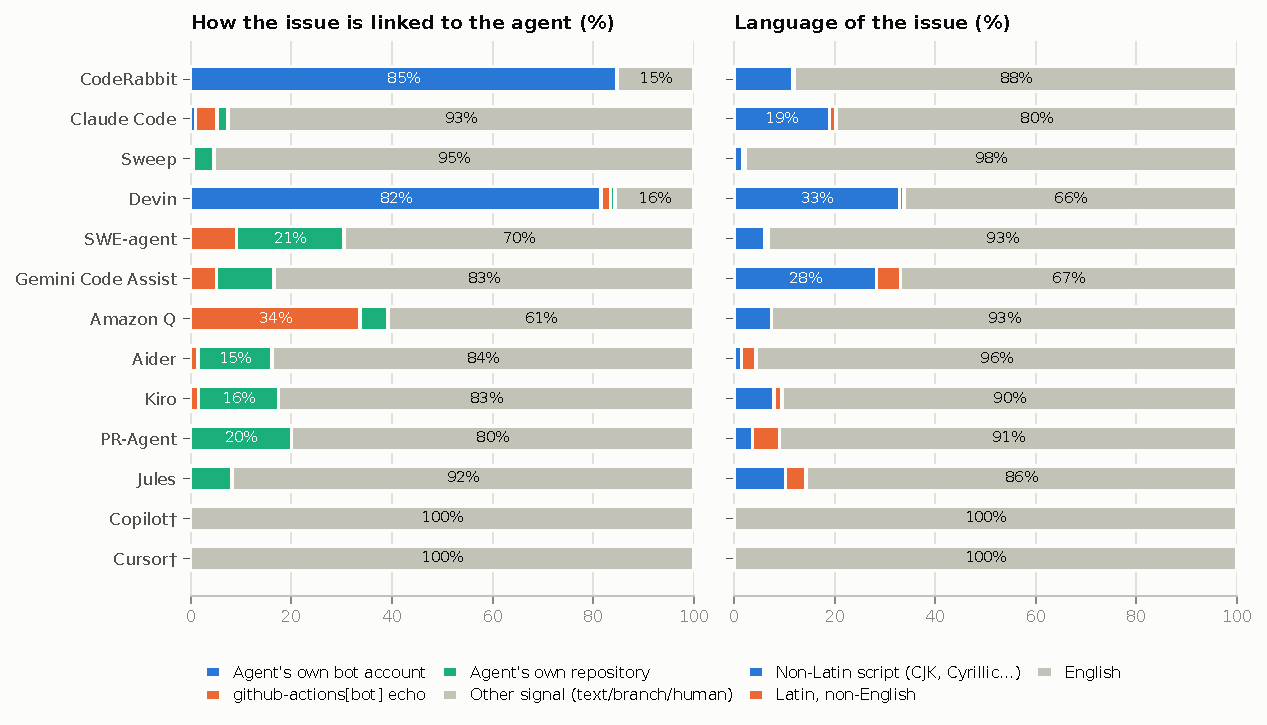
\includegraphics[width=0.86\textwidth]{rq1_F3_attribution_language.pdf}
\caption{How each agent's issues are linked to the agent (left) and their language (right).}\label{fig:rq1attr}
\end{figure*}

\emph{Agent-written issues stay open.} The role of the agent turns out to matter for whether an issue is closed. Within the same agent, issues written by the agent's own bot are closed less often than issues linked to the agent in other ways (Table~\ref{tab:fa}): \DiffCoderabbit{} percentage points for CodeRabbit (95\% CI \DiffCICoderabbit; \(h = \HCoderabbit\), \HEffCoderabbit) and \DiffDevin{} points for Devin (95\% CI \DiffCIDevin; \(h = \HDevin\), \HEffDevin), both significant after Holm correction. Issue age is an obvious alternative explanation, but it does not hold: the bot-written issues are \emph{older} (median \AgeOwnCoderabbit{} against \AgeOtherCoderabbit{} days for CodeRabbit), so they have had more time to be closed, and among issues at least 180 days old the gaps hardly change (\DiffOldCoderabbit{} and \DiffOldDevin{} points). Across all agents, \OwnClosedAll\% of bot-written and \OtherClosedAll\% of other issues are closed. The bot-written issues of the two agents are of different kinds. CodeRabbit's are follow-ups from its reviews (\OwnPRRefAllCoderabbit\% refer to a pull request or review), whereas Devin's mostly describe new tasks (\OwnPRRefAllDevin\%). For CodeRabbit, a plausible reading is that maintainers treat review follow-ups as lower-priority suggestions, in line with developers' reports that unsolicited bot activity feels like noise~\cite{wessel2021disturb}. The data show the association, not its cause.

\begin{table}[t]
\caption{Closure rate (\%, Wilson 95\% CI) of issues written by the agent's own bot and of the agent's other issues}\label{tab:fa}
\centering\footnotesize\setlength{\tabcolsep}{3pt}
\resizebox{\columnwidth}{!}{\begin{tabular}{@{}lccccc@{}}
\toprule
Agent & Own bot & Other & Diff.\ (pp) & z & p\\
\midrule
CodeRabbit & \OwnClosedCoderabbit{} \OwnCICoderabbit & \OtherClosedCoderabbit{} \OtherCICoderabbit & \DiffCoderabbit & \ZCoderabbit & $\PCoderabbit$\\
Devin & \OwnClosedDevin{} \OwnCIDevin & \OtherClosedDevin{} \OtherCIDevin & \DiffDevin & \ZDevin & $\PDevin$\\
\bottomrule
\end{tabular}}
\end{table}

\emph{The labelling illusion.} Labels are GitHub's built-in way to classify and triage issues, and how projects use them is associated with how issues are resolved~\cite{cabot2015labels}. By the usual measure, Sweep is the most-labelled tested agent: \SweepAnyLabel\% of its issues carry a label (95\% CI \SweepAnyLabelCI). Most of these labels, however, are \texttt{sweep} itself (\SweepLabelShare\% of all labels on Sweep's issues), the label a user adds to invoke the agent. Counting only labels that classify the work, Sweep falls to \SweepTriageLabel\% and ranks last of all thirteen agents, a drop of \SweepDrop{} points. Amazon Q (\(-\)\AmazonQDrop{} points) and Jules (\(-\)\JulesDrop) drop too, while no other agent changes by more than \OtherMaxDrop{} points. For trigger-based agents, a label therefore records how the agent was called, not how maintainers organise the work. This adds a new source of noise to labels that are already known to be unreliable as an issue classification~\cite{herzig2013bug}.

\rqsummary{RQ1}{Agents differ most in how their issues are linked to them. For CodeRabbit and Devin, most issues were written by the agent's own bot, and these issues are closed 18--24 percentage points less often than the same agents' other issues, a gap that issue age does not explain. For trigger-based agents such as Sweep, most labels invoke the agent rather than classify the work. Comparisons of ``agent issues'' should therefore separate the role of the agent and remove agent-workflow labels before using labels as data.}


\section{RQ2: Does Time-to-Close Differ Across Agents?}\label{sec:rq2}
\textbf{Motivation.} Time-to-close is a common proxy for how quickly maintainers act on an issue, and it has long been studied as a property of issues~\cite{kikas2016lifetime}. For an adopter, it answers a practical question: do the issues that come with one agent sit idle longer than those of another? It also comes with a pitfall. A third of the issues in the data are still open, and any analysis that uses only closed issues leaves out the slowest ones.

\textbf{Approach.} The first comparison uses the \NRQTwo{} closed issues of the eleven tested agents. Their time-to-close is far from normal: Shapiro--Wilk~\cite{shapiro1965normality} rejects normality for every agent (\(p < 10^{-6}\); skewness \SkewMin\ to \SkewMax), and even after a log transformation it is rejected for \NNonNormalLog{} of the eleven agents. The right tail is long: across the tested agents, the mean time-to-close is \TTCMeanAll{} hours against a median of \TTCMedianAll{} hours (IQR \TTCIQRAll{} h, SD \TTCSDAll{} h), and the Q--Q plots in the replication package show the same pattern for every agent. The comparison therefore uses the Kruskal--Wallis test with \(\varepsilon^2\), Dunn's pairwise test with Holm correction and Cliff's \(\delta\). It is then repeated on all issues of the tested agents with the Kaplan--Meier estimator, which counts an issue that is still open as censored, so that it contributes the time it has been open without being treated as closed. Finally, the main test is repeated on the four sensitivity subsets S1--S4.

\begin{table}[t]
\caption{Time-to-close per agent. Closed issues: count, median in hours with exact 95\% CI, rank. All issues: \% still open, Kaplan--Meier (KM) median in days (n.r.\ = 50\% closed never reached), rank}\label{tab:rq2}
\centering\footnotesize\setlength{\tabcolsep}{2.5pt}
\resizebox{\columnwidth}{!}{\begin{tabular}{@{}lrrcrrrr@{}}
\toprule
& \multicolumn{3}{c}{Closed issues} & \multicolumn{2}{c}{All issues} & \multicolumn{2}{c}{Rank}\\
\cmidrule(lr){2-4}\cmidrule(lr){5-6}\cmidrule(l){7-8}
Agent & n & Median & 95\% CI & Open & KM & Closed & KM\\
\midrule
\inputtab{generated/tab_rq2_ttc.tex}
\bottomrule
\end{tabular}}
\end{table}

\textbf{Results.} \emph{Closed issues.} Time-to-close differs across agents (Kruskal--Wallis \(H = \KWH\), df = \KWdf, \(p = \KWp\)) with a \KWeff{} effect (\(\varepsilon^2 = \KWeps\)). Medians range from \MedPrAgent{} hours for PR-Agent and \MedClaudeCode{} hours for Claude Code to \MedCoderabbit{} hours for CodeRabbit (Table~\ref{tab:rq2}). The overall effect, however, comes from a few agents at the extremes. Only \NSig{} of the 55 pairs of agents differ significantly after Holm correction, and by Cliff's \(\delta\), \NPairsNegligible{} pairs differ negligibly, \NPairsSmall{} slightly, \NPairsMedium{} moderately and \NPairsLarge{} strongly. The largest difference is between Claude Code and CodeRabbit (\(\delta = \DeltaMax\)), and Claude Code takes part in four of the five medium differences. The effect stays medium when issues closed as completed (\(\varepsilon^2 = \EpsCompleted\)) and issues closed as not planned (\(\varepsilon^2 = \EpsNotPlanned\), \NAgentsNotPlanned{} agents with at least ten such issues) are tested separately.

\emph{Robustness.} The effect remains medium without pre-release issues (S1, \(\varepsilon^2 = \EpsSOne\)), on the CodAGE precision subset (S3, \(\varepsilon^2 = \EpsSThree\)) and with one value per agent and repository (S4, \(\varepsilon^2 = \EpsSFour\)), so issues repeated in the same repository do not drive it. It shrinks to small when only human-authored issues are kept (S2, \(\varepsilon^2 = \EpsSTwo\)), which suggests that part of the difference between agents is associated with bot authorship. The ranking of the agents hardly changes in any subset (Spearman \(\rho \geq \RhoSTwo\)).

\begin{figure*}[t]
\centering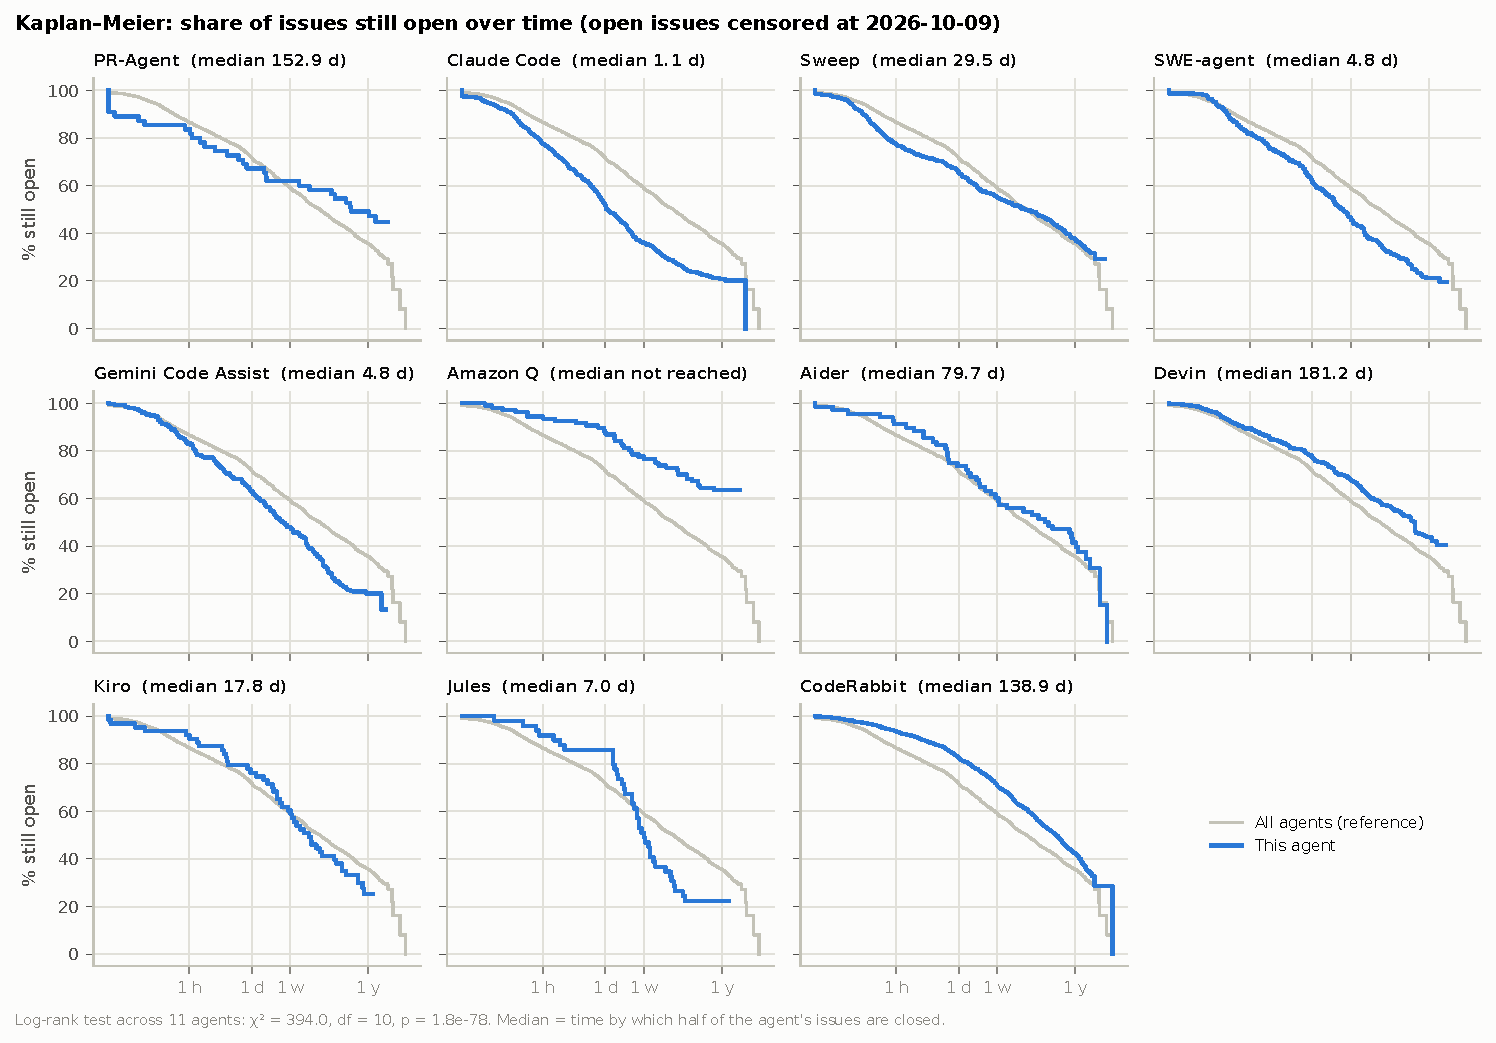
\includegraphics[width=0.86\textwidth]{rq2_R3_kaplan_meier.pdf}
\caption{Kaplan--Meier curves: share of each agent's issues still open over time, with open issues censored. The grey line shows all agents together.}\label{fig:km}
\end{figure*}

\emph{Counting the issues that are still open.} The picture changes once open issues are taken into account (Fig.~\ref{fig:km}). The difference between agents remains significant (log-rank \(\chi^2 = \LRchi\), \(p = \LRp\)), but the two rankings barely agree (Spearman \(\rho = \RankRho\)). PR-Agent, the fastest agent on closed issues, drops to 9th, because \PctOpenPrAgent\% of its issues are still open. Amazon Q falls from 6th to last: \PctOpenAmazonQ\% of its issues are open, so its Kaplan--Meier curve never reaches 50\% closed. Jules moves the other way, from 10th to 4th. Claude Code is fast under both views, 2nd on closed issues and 1st with Kaplan--Meier (median \KMClaudeCode{} days).

\emph{The role of the agent again.} The same bias affects the comparison of bot-written and other issues within an agent. Among \emph{closed} issues, bot-written CodeRabbit issues take longer than other CodeRabbit issues (median \YOwnCoderabbit{} against \YOtherCoderabbit{} hours, \(\delta = \YDeltaCoderabbit\)), but bot-written Devin issues are closed \emph{faster} than other Devin issues (\YOwnDevin{} against \YOtherDevin{} hours, \(\delta = \YDeltaDevin\)). Once open issues are counted, the bot-written issues of both agents are far slower: the Kaplan--Meier median is \YKMOwnCoderabbit{} against \YKMOtherCoderabbit{} days for CodeRabbit and \YKMOwnDevin{} against \YKMOtherDevin{} days for Devin (log-rank, Holm-adjusted \(p = \YLRpCoderabbit\) and \(\YLRpDevin\)). For Devin, then, the closed issues alone would suggest the opposite of what happens to its issues as a whole.

\rqsummary{RQ2}{Time-to-close differs across agents with a medium effect, but mostly at the extremes: 50 of the 55 pairs of agents differ negligibly or slightly. How open issues are handled changes the answer. Ranking agents by their closed issues disagrees with a survival analysis that counts open issues (\(\rho = \RankRho\)), and for Devin the closed issues alone even reverse the comparison between bot-written and other issues. Comparisons of agent speed should use survival analysis rather than closed issues only.}


\section{RQ3: Which Topics Do the Issues Raise?}
\label{sec:rq3}
\textbf{Motivation.} RQ1 and RQ2 show \emph{that} the agents' issues differ; they do not show what the issues are about. Studies of agent pull requests suggest that developers hand agents particular kinds of work, such as refactoring, documentation and testing~\cite{watanabe2025agentic}. If the same holds for issues, topics can explain part of the differences in closure and speed, and they tell maintainers what work to expect from each agent.

\textbf{Approach.} \emph{Corpus.} The topic models cover the \NEnglishTested{} English issues of the eleven tested agents. Each document is the issue title and body after removing code blocks, links, HTML, user mentions, template text (lines repeated verbatim in at least ten issues) and every agent name and signature, so that a topic cannot simply restate the agent label. Tokens were lemmatised and frequent word pairs joined, and only terms were kept that occur in at least ten documents and at most half of them. Documents with fewer than ten tokens were dropped, which leaves \NDocsRQThree{} documents (median \MedTokens{} tokens) and \NVocab{} terms.

\emph{Single LDA runs.} LDA~\cite{blei2003lda} is the most widely used topic model in software-engineering research~\cite{chen2016survey,silva2021topic}, so the analysis started there. It was fitted for \(k = 5\) to 20 topics with three random seeds each, and C\textsubscript{v} coherence~\cite{roder2015coherence} was measured. Coherence hardly changes with \(k\) (\CvMin\ to \CvMax), so it cannot single out one model. A bigger problem is that the topics are not reproducible: when a model is refitted with another seed, at most \SelRepro\% of the topics of the best model (\(k = \SelK\), C\textsubscript{v} = \SelCv) and at most \SingleReproMax\% for any \(k\) reappear, where a topic counts as reappearing if at least seven of its ten top words recur in the matched topic~\cite{greene2014stability}. A topic list from a single run would therefore partly reflect the random seed, a risk that Agrawal et al.\ warned about for software-engineering data~\cite{agrawal2018wrong}.

\emph{Ensemble LDA at two levels.} The study therefore uses Ensemble LDA~\cite{brigl2019ensemble}, which fits many models (here 16) and keeps only the topics that recur across them, with two independent ensembles fitted with different seeds. Under the rule fixed in advance, which chooses the clustering threshold that maximises the number of topics reproduced by both ensembles, \NTopicsH{} topics remain; they form the \emph{headline} level. Two topics are coarse, so the paper also reports a \emph{fine} view: the threshold at which both ensembles find the most topics (\NTopicsF). The researcher defined this second rule after seeing the headline result, so every fine topic is graded by how many of its ten top words recur in the matching topic of the other ensemble: \emph{reproduced} (seven or more), \emph{partly reproduced} (five or six) or \emph{not reproduced} (fewer than five).

\emph{Labels and their validation.} Each topic was labelled after reading its top words and its most representative issues, and the researcher then checked the labels of the fine topics on five random issues per topic, judging for each whether the label describes it. Before the check, the rule was set that a label fails if two or more of its five issues do not fit. A fine topic is interpreted only if it is reproduced \emph{and} its label passes this check.

\emph{Triangulation with BERTopic.} Recent studies of agent pull requests and of issue trackers use BERTopic~\cite{opu2025performance,das2024chatgpt,grootendorst2022bertopic}, which clusters documents by meaning rather than by word co-occurrence. To test whether the conclusions depend on the method, the same documents were also clustered with BERTopic: sentence embeddings~\cite{reimers2019sbert} of the whole issue (long issues are embedded in 150-word chunks that are then averaged), dimensionality reduction with UMAP~\cite{mcinnes2018umap}, and \(k\)-means with as many clusters as the fine view has topics, repeated with three seeds.

\begin{table*}[t]
\caption{RQ3 topics at the headline level (H) and in the fine view (T). Shared = top-10 words that recur in the matching topic of the second, independent ensemble; Prev.\ = share of all topic weight (\%)}\label{tab:rq3}
\centering\footnotesize\setlength{\tabcolsep}{3pt}
\begin{tabular}{@{}l l r r l@{}}
\toprule
& Label & Shared & Prev. & Top words\\
\midrule
\inputtab{generated/tab_rq3_topics.tex}
\bottomrule
\end{tabular}
\end{table*}

\textbf{Results.} \emph{Topics.} At the headline level, the issues split into code maintenance and quality work (H1) and AI and LLM tooling and research (H2), both reproduced across ensembles (Table~\ref{tab:rq3}). In the fine view, two topics meet both conditions for interpretation: testing, review and quality follow-ups (T1; label fits \ValFitOneK{} of \ValFitOneN{} sampled issues) and code-level fixes and refactoring (T4; \ValFitFourK{} of \ValFitFourN). The other three fine topics are not interpreted. T2, whose words suggest implementation plans and integration phases, does not recur in the second ensemble. T3 and T5 recur only partly, and their labels failed the check (\ValFitThreeK{} and \ValFitFiveK{} of 5 issues fit): the sampled issues ranged from a thermostat bug to a payment-channel problem, so these two word lists do not describe a coherent kind of work.

\emph{Topics depend on the agent.} The topics of an agent's issues depend on the agent (Fig.~\ref{fig:rq3heat}). The association is \EffTHMain{} at the headline level (V = \VTHMain) and at the border between medium and large in the fine view (V = \VTFMain, where the threshold for a large effect is 0.25). It holds for human-authored issues only (S2, V = \VTFSTwo), on the precision subset (S3, V = \VTFSThree) and when the documents of the non-reproduced topic are left out (V = \VTFStable). It is much weaker, though still significant, when the ensemble is refitted on a corpus that also contains very short issues of five to nine tokens: the topics then change, and V drops to \VTFFive{} in the fine view and \VTHFive{} at the headline level.

\begin{figure*}[t]
\centering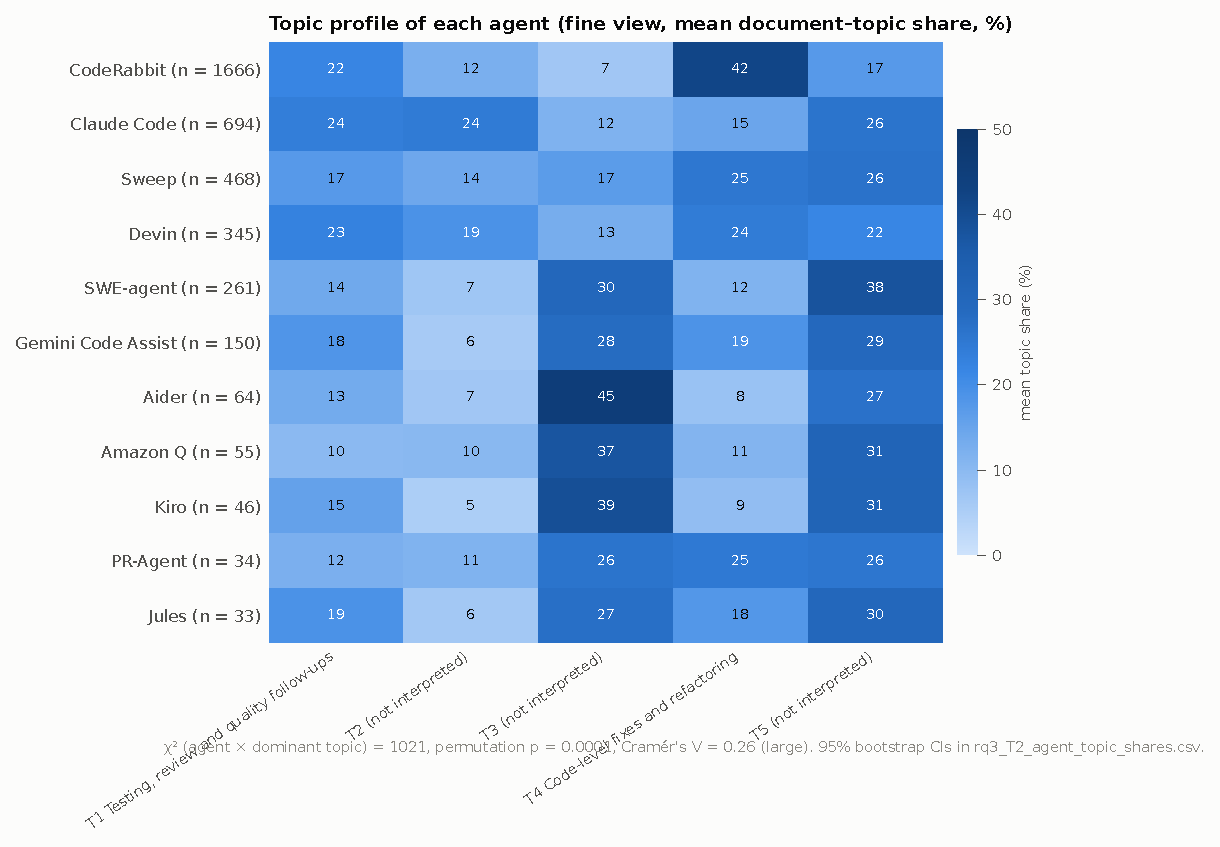
\includegraphics[width=0.62\textwidth]{rq3_R2_agent_topic_heatmap.pdf}
\caption{Topic profile of each agent in the fine view: mean share of each topic in the agent's issues (\%).}\label{fig:rq3heat}
\end{figure*}

\emph{Which agents drive it.} Adjusted residuals beyond \(|z| = \ZCritFine\) (Bonferroni) count as significant, and they are read only for the interpreted topics. CodeRabbit shows the clearest pattern. Its issues are strongly over-represented in code-level fixes (\(z = \ResCodeRabbitCode\), and \(z = \ResSThreeCodeRabbitCode\) on the precision subset), which make up \ShareCodeCodeRabbit\% of the topic weight of its issues (95\% bootstrap CI \ShareCodeCodeRabbitCI), and it wrote \CodeTopicShareCodeRabbit\% of the issues dominated by this topic although it accounts for \DocShareCodeRabbit\% of the documents. The pattern comes from the issues CodeRabbit writes itself: \CodeRabbitOwnPRRef\% of them refer to a pull request or a review, and code-level fixes make up \CodeShareOwnCodeRabbit\% of their topic weight, against \CodeShareOtherCodeRabbit\% for CodeRabbit's other issues. These are the issues that RQ1 showed are often left open.

\emph{Triangulation.} BERTopic is far more stable than LDA: all of its topics recur across seeds (adjusted Rand index between seeds \BTAriMin\ to \BTAriMax). It confirms the main conclusion: topics depend on the agent, with a \BTEff{} effect (V = \BTV, and \BTVMin\ to \BTVMax\ across seeds). On BERTopic's own topics, CodeRabbit is again over-represented in code-level work (\(z = \BTResCodeRabbitCode\)). The two methods divide the corpus differently, however. Matched topics share few top words (mean Jaccard \TriWordJ), and agreement at the level of single issues is low (adjusted Rand index \TriARI; \TriSame\% of issues fall in the matched topic).

\emph{Topics and time-to-close.} Time-to-close differs only slightly between the fine topics (\(\varepsilon^2 = \TopicKWeps\), \TopicKWeff; log-rank \(p = \TopicLRp\)). Code-level fixes have the longest Kaplan--Meier median (\KMDaysCode{} days) and build and workflow issues the shortest (\KMDaysWorkflow{} days). Because two-thirds of the code-level issues come from CodeRabbit, this difference cannot be separated from the agent.

\rqsummary{RQ3}{Agents raise different kinds of work. The association holds under two topic models, across seeds and on the S2 and S3 subsets, but it weakens when very short issues are included. The clearest case is CodeRabbit: its own issues are follow-ups from pull-request reviews, code-level fixes, a topic that is reproduced and whose label passed manual validation, are their largest topic, and CodeRabbit's issues lean towards code-level work under both topic models. Only two of the five fine topics, however, are both reproducible and correctly labelled, and LDA and BERTopic divide the same issues differently. Topic-modelling studies of agent artefacts should therefore check topic stability, validate topic labels by hand, and confirm their conclusions with a second method before interpreting individual topics.}


\section{Discussion}\label{sec:discussion}
The three research questions point in the same direction. The agents differ, but much of the difference lies in the role the agent plays in an issue, and in whether the analysis looks only at issues that were closed. The findings matter to three audiences in different ways.

\textbf{For maintainers.} Issues written by an agent's own bot are, for both agents where a comparison is possible, closed far less often than the agent's other issues (RQ1). For the review agent CodeRabbit, these are follow-ups from its pull-request reviews, often code-level suggestions (RQ3). Projects that enable a review agent should therefore plan for this stream of issues: route them to a person who triages them, group them, or close them automatically after a set time. Otherwise they accumulate as backlog, the kind of bot activity that developers already describe as noise~\cite{wessel2021disturb}. Maintainers should also not read the labels on issues of trigger-based agents such as Sweep as a classification of the work: there, most labels only invoke the agent (RQ1).

\textbf{For agent developers.} An agent that opens its own issues creates work for maintainers, and a large share of these issues stays open. Developers of such agents could make their issues easier to act on, for example by linking each issue to the review comment and the lines of code it comes from, by stating a priority, or by closing an issue once the underlying code has changed. Agents could also mark clearly how they are involved in an issue. That would reduce the ambiguity that currently forces datasets to attribute issues with heuristics~\cite{ghaleb2026codage,ghaleb2026fingerprinting}.

\textbf{For researchers.} ``AI coding agent'' is not one kind of actor. In the hand-checked sample, the agent had written fewer than a third of the issues correctly attributed to it, and in half it was only mentioned. Four consequences follow for studies that compare agents. First, they should record and report the role of the agent in each artefact, because pooling issues an agent wrote with issues that merely mention it can produce differences that belong to the role, not the agent (RQ1). They should also validate the attribution by hand on a sample; in this study, most wrong attributions came from text signals. Second, they should compare speed with survival analysis: in this study, the ranking of agents by closed issues barely agreed with the censoring-aware ranking, and for one agent the closed issues even reversed a comparison (RQ2). Third, they should remove agent-workflow labels before treating labels as data, adding to known problems with label quality~\cite{herzig2013bug}. Fourth, they should test whether their topics are reproducible, check the topic labels on sample issues, and confirm the results with a second method (RQ3): on this corpus, only two of five fine topics passed both the stability test and the label check. Single LDA runs were not reproducible on this corpus, which echoes earlier warnings~\cite{agrawal2018wrong}, and two reasonable topic models divided the same issues differently while agreeing on the agent-level conclusions.


\section{Threats to Validity}\label{sec:threats}
The four classic types of threats~\cite{wohlin2012experimentation} are discussed below, each with the steps taken to reduce it.

\textbf{Construct validity.} The main construct, the agent behind an issue, comes from a heuristic attribution that its authors describe as a candidate with false positives by design~\cite{ghaleb2026codage}. It was kept as given, as the study brief requires, but the study reports for every agent how its issues are linked to it, repeats the key tests on the high-precision subset (S3) and after removing \NPreRelease{} issues created before the agent's public release (S1), and the researcher validated a stratified random sample of 99 issues by hand (nine per tested agent, rated blind). In this sample, \ValCorrectPct\% of the attributions are correct (95\% CI \ValCorrectCI), ranging from \ValCorrectAiderK{} of \ValCorrectAiderN{} for Aider to all nine for Claude Code, Devin and Kiro. Most errors (\ValWrongOtherK{} of \ValWrongOtherN) come from text signals, for example the word ``Raider'' matched as Aider, or the ordinary word ``sweep'' matched as the agent Sweep, which is the weakness the dataset's documentation warns about. The own-bot flag, on which the closure gap in RQ1 rests, was right for all \ValOwnBotPrecisionK{} issues it flagged, but it caught only \ValOwnBotRecallK{} of the \ValOwnBotRecallN{} sampled issues that the agent itself had written (\ValOwnBotRecallPct\%, 95\% CI \ValOwnBotRecallCI). It misses, for example, issues that people posted with a ``Generated with Claude Code'' footer. RQ1 therefore compares issues opened by the agent's own bot account with all of the agent's other issues, a group that also contains some agent-written and some misattributed issues. The rule was kept unchanged rather than tuned after seeing the validation. Some attributed issues are automated content that merely mentions an agent, for example \NDigest{} daily paper digests posted by \texttt{github-actions[bot]} that mention SWE-agent or Aider; the S3 subset excludes all but \NDigestInSThree{} of them. Time-to-close measures whether an issue was closed, not whether the problem was solved, and an issue closed as \emph{not planned} is not a fix; each closure reason is therefore also tested separately. The label categories come from published rules defined for this study, the language flag is a heuristic that was checked by hand on 40 issues (\ValNonEnK{} of \ValNonEnN{} flagged non-English and \ValEnK{} of \ValEnN{} flagged English issues were classified correctly), and the RQ3 topic labels are an interpretation of word lists and sample issues. They were checked by hand on five issues per topic, and only the two fine topics whose labels passed are interpreted (Section~\ref{sec:rq3}). All judgements were made by the author alone; the blind samples and the answers are in the replication package, so that others can re-rate them.

\textbf{Internal validity.} This is an observational study, so all results are associations, not effects of the agents. Bot authorship is confounded with the agent: CodeRabbit and Devin issues are mostly bot-written and the others are not. Comparisons within the same agent (RQ1, RQ2) and the human-authored subset (S2) address this; in S2, the agent effect on time-to-close shrinks from medium to small. Issues of different agents also differ in age; age was checked and does not explain the closure gap, and the survival analysis accounts for the different time each issue has been open. Many issues from one repository could inflate the evidence, but no repository holds more than \TopRepoMax\% of any tested agent's issues, and one value per agent and repository (S4) gives the same effect size.

\textbf{External validity.} The data are one extract of public GitHub issues for \NAgents{} agents, without any filter for repository popularity or activity, so personal and toy projects are included. The agents change quickly, and the results describe them as they were used in this period. Five of the tested agents have fewer than 110 issues, which limits what can be said about them individually, and RQ3 covers English issues only.

\textbf{Conclusion validity.} Time-to-close is heavily skewed, so all tests are rank-based, with an effect size reported for every test and a confidence interval with every rate and median. Families of tests are Holm-corrected, and sparse tables are tested by permutation. Statistical claims require at least 30 closed issues per agent; Selvanayagam and Ghaleb used a stricter threshold of 50~\cite{selvanayagam2026aitoai}, which would remove five of the agents studied here. Single LDA runs were not reproducible on this corpus, so the topics come from Ensemble LDA, graded by their reproducibility, and the agent--topic association is confirmed with BERTopic. The fine-view rule and the ``partly reproduced'' grade were defined after the headline result; this is stated explicitly, and the headline level uses only the rule fixed in advance. The agent--topic association becomes weaker when very short issues are added. Finally, in gensim~4.3 the setting \(\eta = \)``auto'' does not change the fitted topics, so fixed values of \(\eta\) were tuned instead. To guard against errors, every number in this report is generated from the result files, and independent scripts re-compute the key statistics.


\section{Conclusion and Future Work}\label{sec:conclusion}
This study compared \NIssues{} GitHub issues attributed to \NAgents{} AI coding agents on their volume, state and labelling, their time-to-close and their topics. The agents differ, but the clearest difference is in the role the agent plays: some agents write their own issues, others are triggered by humans or merely mentioned. That role is associated with what happens to the issue. Issues written by an agent's own bot are closed less often than the same agent's other issues; for the review agent CodeRabbit, these are follow-ups from its reviews. Comparing agents by their closed issues alone gives a misleading ranking, and survival analysis corrects it. Topics differ by agent under two topic models, even though the two models divide the corpus differently.

\textbf{Future work.} Three directions follow. \emph{Following issues to their outcome:} linking agent-written issues to the pull requests and commits that address them would show whether open issues are ignored or resolved without being closed. \emph{A human baseline:} comparing agent-attributed issues with human issues in the same repositories would show which differences are specific to agents. \emph{Better attribution:} a larger hand-labelled sample, rated by more than one person, would allow the attribution to be corrected rather than only checked.


\section*{Ethics and Disclosures}
\textbf{Ethics.} The study uses only public GitHub data provided for the course. The researcher followed the Menlo Report principles~\cite{dittrich2012menlo} and the guidance of Gold and Krinke on mining software repositories~\cite{gold2022ethics}: no attempt was made to identify individuals, only aggregates are reported, and no user accounts are named in this report. Agent names are product names. The replication package does not redistribute the dataset.

\textbf{Use of generative AI.} The researcher used Claude (Anthropic) as an assistant for the literature search, for writing and checking the code scripts, and for drafting and editing the text. All study decisions and the manual validation were the researcher's own; every reported number is generated from the result files and independently re-checked, and the researcher reviewed and is responsible for the entire content.


\section*{Data and Replication Package}
The replication package is publicly available at \url{https://github.com/Invincible1811/same-label-different-work}. It contains all scripts (\texttt{src/}), the verification checks (\texttt{checks/}), every result table and the data behind every figure as CSV files, a manifest with SHA-256 hashes, exact library versions, the manual-validation samples and answers, the decision log, and a step-by-step guide. The course dataset is not redistributed; placing it in \texttt{data/raw/} and running \texttt{run\_all.sh} reproduces all results. CodAGE is licensed under CC~BY~4.0 and builds on GH~Archive.


\bibliographystyle{IEEEtran}
\bibliography{refs}
\end{document}
